% !TEX program = xelatex
\documentclass[aspectratio=169]{beamer}

% --- Enable notes ---
% \setbeameroption{show notes} % allow \note{} content

% --- Show notes on second screen (right of main slides) ---
% \setbeameroption{show notes on second screen=right}

\usepackage{xcolor}
\usepackage{listings}
\usepackage[english]{babel}
\usepackage{fontspec}

\usepackage{amsmath}
\usepackage{amssymb}
\usepackage{siunitx}
\usepackage{pifont}
\usepackage{caption}


\usepackage{tikz}
\usepackage{tikzpagenodes}
\usetikzlibrary{shapes,calc,decorations.pathreplacing,decorations.pathmorphing,arrows.meta,shapes.geometric,shapes.callouts}
\usetikzlibrary{positioning,fit,patterns,trees,backgrounds,matrix,overlay-beamer-styles,tikzmark,fadings}
 
% Shared palette, derived from the grid-index figures.
\definecolor{color1}{HTML}{4357AD}
\definecolor{color2}{HTML}{48A9A6}
\definecolor{color3}{HTML}{E4DFDA}
\definecolor{color4}{HTML}{D4B483}
\definecolor{color5}{HTML}{C1666B}

\def\pagecolor{color4}
\def\cellcolor{black}
\def\pagebuffercolor{color4}
\def\volumecolor{color2}
\def\imbalancecolor{color4}
\def\overheadcolor{color5}
\def\ttopacity{1}

\tikzset{
  my callout style/.style={
    draw=none, rectangle callout, anchor=pointer,
    callout relative pointer={(320:1.5cm)},
    rounded corners, align=center, opacity=\ttopacity
  },
  overlay callout/.style={
    draw=none, rectangle callout,
    callout relative pointer={(320:1.5cm)},
    rounded corners, align=center, opacity=\ttopacity
  },
  iconW/.store in=\iconW, iconW=4cm,
  iconH/.store in=\iconH, iconH=4cm,
  barrel/.style={
    draw, gray!70!black, fill=\volumecolor,
    shape=cylinder, shape border rotate=90,
    aspect=0.35, minimum width=9mm, minimum height=11mm, line width=0.6pt
  },
  leafbox/.style={
    draw=gray!70!black, fill=\overheadcolor, rounded corners=0.9pt,
    minimum width=4mm, minimum height=4mm, line width=0.5pt
  },
  gridcell/.style={
    draw=gray!70!black, fill=color3, rounded corners=0.9pt,
    minimum width=4mm, minimum height=4mm, line width=0.5pt
  },
  beam/.style={line width=0.9pt},
  loadL/.style={
    draw=gray!70!black, fill=\imbalancecolor, line width=0.6pt,
    minimum width=8mm, minimum height=7mm
  },
  loadR/.style={
    draw=gray!70!black, fill=\imbalancecolor, line width=0.6pt,
    minimum width=5mm, minimum height=5mm
  },
  fulcrum/.style={draw, fill=black!15, line width=0.6pt},
  iconbox/.style={
    minimum width=\iconW, minimum height=\iconH,
    inner sep=0, outer sep=0, draw=none
  },
  halo arrow/.style={
    ->, >=Stealth, line width=2pt, draw=black, line cap=round
  }
}


\usetheme[numbering=fraction]{metropolis}

\usetheme{default}
\setbeamercolor{background canvas}{bg=white}
\setmainfont{Source Sans Pro}

\title{Index Intersection\\for High-Dimensional Range Queries}
\author{\textbf{Max Berens} \& Jens Teubner}
\date{52nd International Conference on Very Large Data Bases $\cdot$ Boston, MA, USA $\cdot$ 2026}

\begin{document}
\maketitle

% Main deck
\begin{frame}{\textit{Motivation} --- High-Dimensional Range Queries}
%% This slide briefly sketches the problem setting and mentions the CERN as the motivational context.
%% Key points: high table dimensionality, high table cardinality, high query selectivity, rectangular ad-hoc range queries, storage space consumption
%% Assumption: It would be worth doing (secondary) indexing, but the indices are too expensive
%% Assumption: At this scale, knowing the selectivity of a query is beneficial in its own right
\input{figures/motivation-flow}
\end{frame}

\begin{frame}{\textit{Motivation} --- Indexing: 1-for-All vs. 1-for-Every\ldots?}
%% This slide compares the two extremes of secondary indexing: one index for all attributes vs. one index for every attribute (`bitmap indices'). It motivates the need for a more flexible design space, which is then explored in the next slide.
%% Lastly, it suggests exploring the space in between the two extremes, which is then further explained in the next slide.
%% Key points: the two extremes and plausible drawbacks (i.e., why they are infeasible in practice), the new idea/our core contribution
\input{figures/index-design-space}
\end{frame}

\begin{frame}{Team-based Indexing: Between the Extremes}
%% Illustrative uniform workload: the Grid Index and its bin precision are deliberately
%% introduced on the following slide. With unequal predicate selectivities, composition matters.
\input{figures/team-indexing-flow}
\end{frame}

\begin{frame}[fragile]{\textit{Methodology} --- Grid Index for a Single Team}
%% Some methodology, mostly to motivate the usage the grid index as an easily to understand and CONFIGURABLE index data structure
%% The figure also introduces the general procedure of a secondary approach, and teases trade-offs
%% It should become clear, how the parameters induce interesting trade-offs, which govern how effective index intersection can become
%% Procedure:
%  \item[1)] For all indices: Map the query rectangle to relevant "leafs"
%  \item[2)] Optimise the ``query'' plan
%  \item[3a)] Fetch relevant leafs
%  \item[3b)] Combine leafs/index intersection
%  \item[4)] Fetch actual candidate rows
%% Key points: grid index, procedure, trade-offs (treaser), configurability and parameters

% Uncomment the following block to restore the original, animated grid-index draft.
\begin{columns}
\column{0.4\textwidth}
% \centering
% {\scriptsize Data Space}
\only<1>{
  \begin{figure}
      \centering
      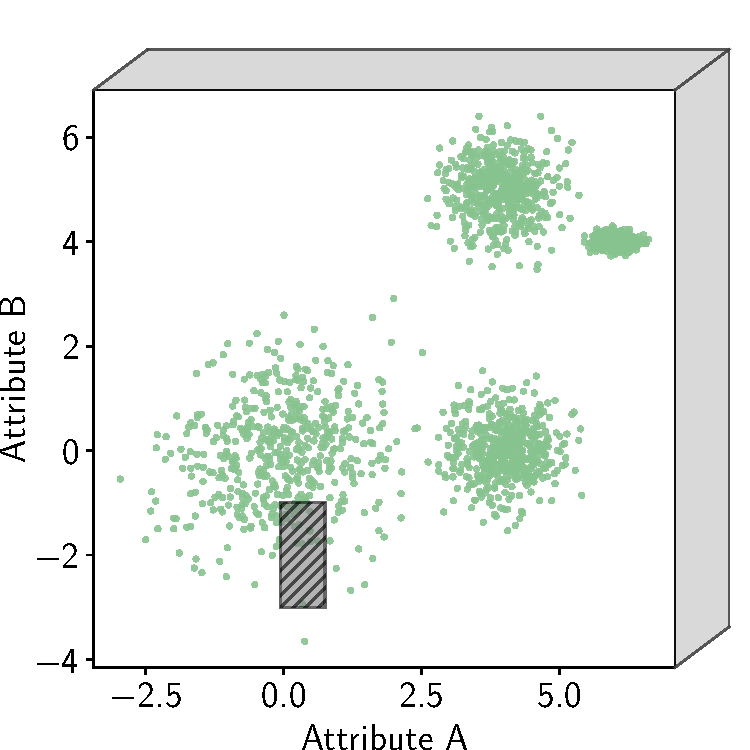
\includegraphics[width=\textwidth]{figures/grid_index_plain}
  \end{figure}
}
\only<2-3>{
    \begin{figure}
        \centering
        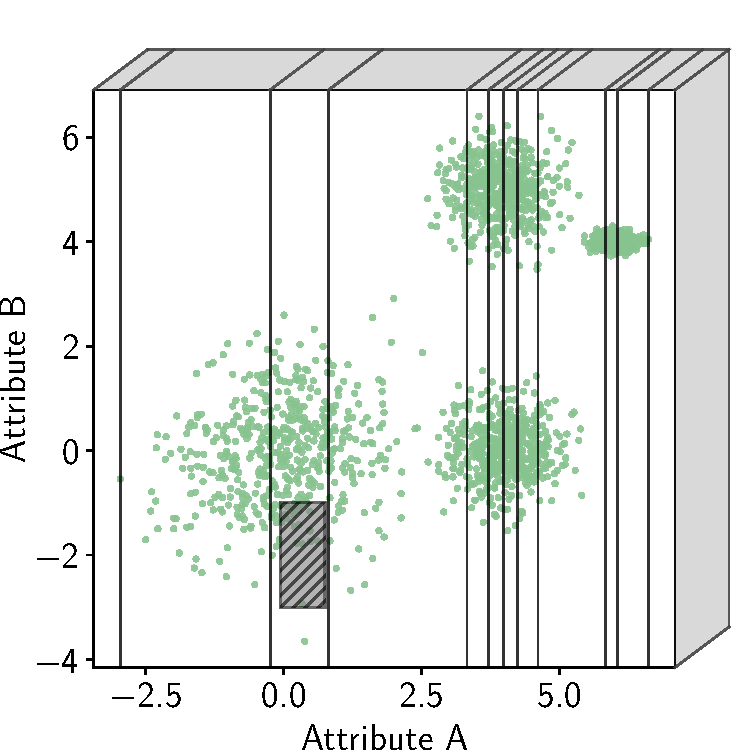
\includegraphics[width=\textwidth]{figures/grid_index_1D}
    \end{figure}
}
\only<4>{
    \begin{figure}
        \centering
        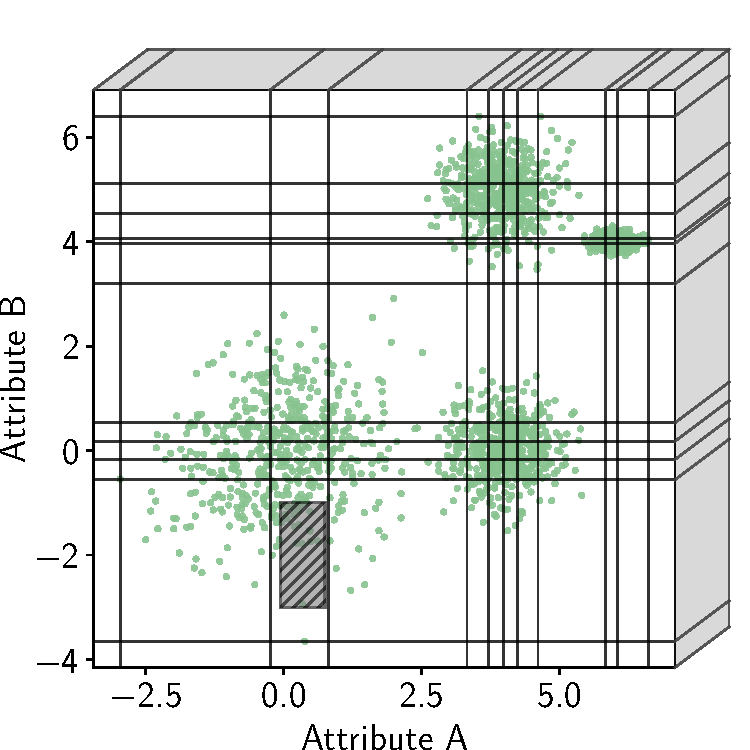
\includegraphics[width=\textwidth]{figures/grid_index_2D}
    \end{figure}
}
\only<5->{
    \begin{figure}
        \centering
        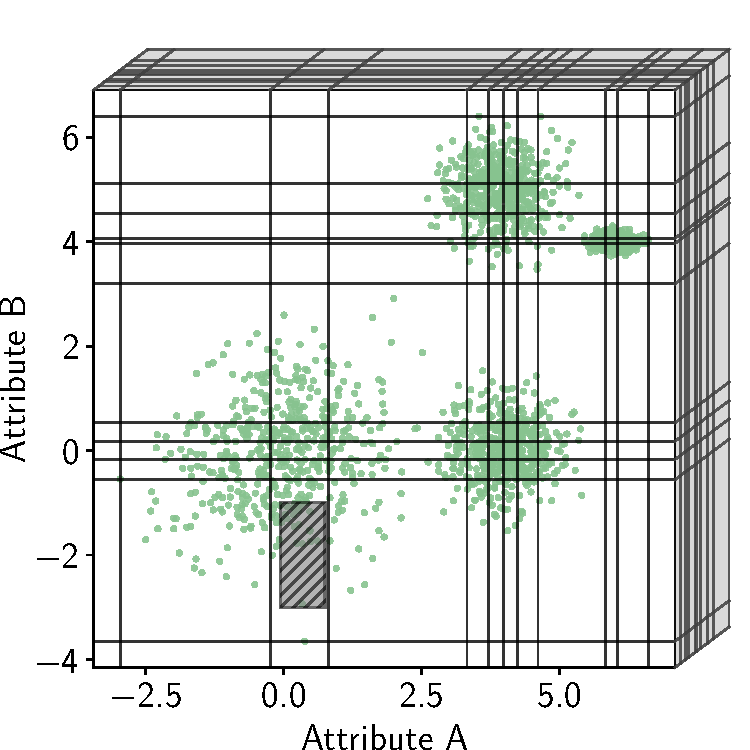
\includegraphics[width=\textwidth]{figures/grid_index_3D}
    \end{figure}
}
\column{0.6\textwidth}
\uncover<2->{
  \begin{tikzpicture}[x=1mm,y=1mm]
    \def\gshift{1.4}%
    \def\goffset{5}%
    \def\goffsetY{14}%
    \def\cellsize{4.5}%
    \def\npages{7}
    \def\pw{9}
    \def\ph{6}
    \def\headerh{3}
    \def\payloady{1}
    \def\payloadh{\ph-\headerh-1}
    \newcommand{\LeafGrid}[7]{%
      \begin{scope}[shift={({#6},{#7})}]
        \pgfmathtruncatemacro{\R}{#2}
        \pgfmathtruncatemacro{\C}{#3}
        \foreach \r in {1,...,\R}{
          \foreach \c in {1,...,\C}{
            \pgfmathsetmacro{\x}{(\c-1)*#4}
            \pgfmathsetmacro{\y}{(\R-\r)*#5}
            \node[gridcell] (#1-r\r-c\c) at (\x,\y) {$\cdot$};
          }
        }
      \end{scope}%
    }
    % Cheaper stand-in for \LeafGrid: only draws the top row and right column
    % (the "rim") of the grid. Used for back layers of the 3D stack that are
    % almost entirely occluded by the layers in front of them, so drawing the
    % full R x C grid of nodes would be wasted rendering time.
    \newcommand{\LeafGridRim}[7]{%
      \begin{scope}[shift={({#6},{#7})}]
        \pgfmathtruncatemacro{\R}{#2}
        \pgfmathtruncatemacro{\C}{#3}
        \foreach \c in {1,...,\C}{
          \pgfmathsetmacro{\x}{(\c-1)*#4}
          \pgfmathsetmacro{\y}{(\R-1)*#5}
          \node[gridcell] (#1-r1-c\c) at (\x,\y) {$\cdot$};
        }
        \foreach \r in {2,...,\R}{
          \pgfmathsetmacro{\x}{(\C-1)*#4}
          \pgfmathsetmacro{\y}{(\R-\r)*#5}
          \node[gridcell] (#1-r\r-c\C) at (\x,\y) {$\cdot$};
        }
      \end{scope}%
    }
    \pgfmathtruncatemacro{\N}{\npages}
    \foreach \i in {1,...,\N} {
        \pgfmathsetmacro{\x}{(\i-1)*\pw}
        \draw (\x,0) rectangle ++(\pw,\ph);
        \ifdim \headerh pt>0pt
        \fill[black!8] (\x,\ph-\headerh) rectangle ++(\pw,\headerh);
        \node[font=\scriptsize\bfseries] at (\x+0.5*\pw,\ph-0.5*\headerh) {Page \i};
        \fi
    }

    \node[text=black, font=\bfseries] at (-4.5,14.3) {Grid:};
    \node[text=black, font=\bfseries] at (-6,\ph/2.0) {SSD:};
    \node[text=black, font=\bfseries] at ({(\N+0.5)*\pw},\ph/2.0) {\ldots};

    \newcommand{\TapeSegment}[3]{%
        \pgfmathsetmacro{\start}{#2-1}
        \pgfmathsetmacro{\L}{#3}
        \pgfmathsetmacro{\nfull}{floor(\L)}
        \pgfmathsetmacro{\rem}{\L-\nfull}
        \foreach \k in {0,...,\nfull} {
        \ifnum \k<\nfull
            \pgfmathsetmacro{\xx}{(\start+\k)*\pw}
            \fill[#1] (\xx,\payloady) rectangle ++(\pw,\payloadh);
        \fi
        }
        \ifdim \rem pt>0pt
        \pgfmathsetmacro{\xrem}{(\start+\nfull)*\pw}
        \pgfmathsetmacro{\wrem}{\rem*\pw}
        \fill[#1] (\xrem,\payloady) rectangle ++(\wrem,\payloadh);
        \fi
    }
    \uncover<5->{
      % Back layers are almost fully covered by the layers drawn in front of
      % them, so only their top-row/right-column rim needs to be rendered.
      \foreach \shift in {9,8,...,3} {
        \pgfmathsetmacro{\offset}{\goffset + \shift*\gshift}
        \pgfmathsetmacro{\offsetY}{\goffsetY + \shift*\gshift}
        \LeafGridRim{arr1}{10}{10}{\cellsize}{\cellsize}{\offset}{\offsetY}
      }
      % The front two layers are fully visible, so draw them completely.
      \foreach \shift in {2,1} {
        \pgfmathsetmacro{\offset}{\goffset + \shift*\gshift}
        \pgfmathsetmacro{\offsetY}{\goffsetY + \shift*\gshift}
        \LeafGrid{arr1}{10}{10}{\cellsize}{\cellsize}{\offset}{\offsetY}
      }
    }
    \uncover<4->{\LeafGrid{arr1}{9}{10}{\cellsize}{\cellsize}{\goffset}{\goffsetY+\cellsize}}
    \LeafGrid{arr1}{1}{10}{\cellsize}{\cellsize}{\goffset}{\goffsetY}
    \coordinate (refcellcoord) at (\goffset+\cellsize, \goffsetY);
    \only<2>{
      \TapeSegment{\pagecolor}{1}{3.6}
      \TapeSegment{\pagecolor}{5}{2.8}
      \node[gridcell,fill=\pagecolor] (refcell) at (refcellcoord) {$\cdot$};
    }
    \uncover<3->{
      \node[gridcell,fill=color5] (refcell) at (refcellcoord) {$\cdot$};
    }
    \only<3>{
      \TapeSegment{\pagecolor}{1}{3.6}
      \TapeSegment{color5}{5}{2.8}
      \draw[halo arrow] (refcellcoord) to[out=60,in=40,looseness=0.95] ($(refcellcoord)+(30,-8)$);
    }
    \only<4>{
      \TapeSegment{\pagecolor}{1}{1.6}
      \TapeSegment{color5}{3}{0.8}
      \draw[halo arrow] (refcellcoord) to[out=50,in=50,looseness=0.95] ($(refcellcoord)+(13,-8)$);
      \TapeSegment{\pagecolor}{4}{1.8}
      \TapeSegment{\pagecolor}{6}{1.15}
    }
    \only<5->{
      \TapeSegment{\pagecolor}{1}{0.6}
      \TapeSegment{color5}{2}{0.8}
      \draw[halo arrow] (refcellcoord) to[out=40,in=60,looseness=0.95] ($(refcellcoord)+(5.2,-8)$);
      \TapeSegment{\pagecolor}{3}{0.1}
      \TapeSegment{\pagecolor}{4}{.2}
      \TapeSegment{\pagecolor}{5}{1.15}
      \TapeSegment{\pagecolor}{7}{.15}
    }
  \end{tikzpicture}
}
\end{columns}

\begin{tikzpicture}[remember picture,overlay]
  \only<2>{\node[overlay callout,draw,fill=color1!50,anchor=pointer,callout relative pointer={(210:0.8cm)}] at ($(current page text area.east)+(-2.2cm,-3.85cm)$) {\textbf{``Leaf''}};}
  \uncover<2-3>{\node[overlay callout,draw,fill=color2!60,anchor=pointer,callout relative pointer={(210:1.7cm)}] at ($(current page text area.north east)+(-4cm,-6cm)$) {$\mathbf{b^d=10^1}$ cells};}
  \only<4>{\node[overlay callout,draw,fill=color2!60,anchor=pointer,callout relative pointer={(210:1.7cm)}] at ($(current page text area.north east)+(-4cm,-6cm)$) {$\mathbf{b^d=10^2}$ cells};}
  \only<5>{\node[overlay callout,draw,fill=color2!60,anchor=pointer,callout relative pointer={(210:1.7cm)}] at ($(current page text area.north east)+(-4cm,-6cm)$) {$\mathbf{b^d=10^3}$ cells};}
  \uncover<3->{
    \draw[halo arrow] ($(current page text area.south west)+(1.9cm,1.8cm)$) to[out=40,in=160,looseness=0.95] ($(current page text area.south west)+(6cm,1.35cm)$);
    % \node[overlay callout,fill=color1!70,anchor=pointer,callout relative pointer={(220:1.3cm)}] at ($(current page text area.north east)+(-2cm,-7.3cm)$) {SSD};
  }
\end{tikzpicture}
\end{frame}

\begin{frame}{Combining multiple Teams}
%%% This slide illustrates how a bunch of selected leafs across multiple Teams imply a set algebra expression and also a query plan for the execution of the intersection.
\only<1>{
    \begin{align*}
    \Bigl(\,\bigcup \text{IDX}_1(i)\Bigr)
        \cap \Bigl(\,\bigcup \text{IDX}_2(j)\Bigr)
        \cap \Bigl(\,\bigcup \text{IDX}_3(k)\Bigr)\\
    \end{align*}
}
\input{figures/team-combination-plan}
\end{frame}

\begin{frame}{Trade-Off: Overhead vs. Volume}
%%% This slide presents results and directly shows the trade-off between accessed data volume, the per-leaf cost explosion and the respective runtime for various "configurations" of our toy index data structure.
%%% Parameter variations indicate how "precision" and "Team size (dimensionality per index)" impact performance.
%%% We also see that per-predicate selectivity impacts access volume, too.
%%% Moreover, we see the differences across random Team compositions for the same "configuration".
\only<1>{
\begin{columns}
\column{0.6\textwidth}
\begin{figure}
    \centering
    \includegraphics[width=\textwidth]{figures/generated/vol_vs_overhead_comparison_1}
\end{figure}
\column{0.4\textwidth}
Table/Index:
\begin{itemize}
    \item $16$ Attributes, $1.22$ B tuples
    \item $\approx 150$ GB
    \item $10^d$ grid per Team
\end{itemize}
\vfill
Queries:
\begin{itemize}
\item \textbf{Selective}: $0.2$ per pred.
\item \textbf{Less Sel.}: $0.2$--$0.8$ per pred.
\end{itemize}
\end{columns}
}
\only<2>{\centering\includegraphics[height=0.82\textheight]{figures/generated/vol_vs_overhead_comparison_2}}
\only<3>{\centering\includegraphics[height=0.82\textheight]{figures/generated/vol_vs_overhead_comparison_3}}
\only<4>{\centering\includegraphics[height=0.82\textheight]{figures/generated/vol_vs_overhead_comparison_4}}
\only<5>{\centering\includegraphics[height=0.82\textheight]{figures/generated/runtime_comparison_1}}
\only<6>{\centering\includegraphics[height=0.82\textheight]{figures/generated/runtime_comparison_2}}
\end{frame}

\begin{frame}{Storage Costs}
\centering\includegraphics[height=0.82\textheight]{figures/generated/storage_comparison}
\end{frame}
\begin{frame}{Dimensional Scaling}
%%% Here we show that we indeed scale linearly out to high dimensional queries (85 dimensions).
%%% We also show the trade-off between selectivity (per attribute) and runtime, and compare the runtime with a hypothetical VA-file scan (which is ideally bound by PCIe bandwidth).
%%% The cross overpoint between VA file style access and inverted access depends mostly on random vs. sequential access speeds
%%% (Lastly, we show the impact of using correlation in Team composition over random Teams, which causes both degradation and improvement.)
\only<1>{\centering\includegraphics[height=0.8\textheight]{figures/generated/dimensional_scaling_comparison_1}}
\only<2>{\centering\includegraphics[height=0.8\textheight]{figures/generated/dimensional_scaling_comparison_2}}
\only<3>{\centering\includegraphics[height=0.8\textheight]{figures/generated/dimensional_scaling_comparison_3}}
\only<4>{\centering\includegraphics[height=0.8\textheight]{figures/generated/dimensional_scaling_comparison_4}}
\begin{tikzpicture}[remember picture,overlay]
    
		% \node[overlay callout,draw,fill=color1!70,anchor=pointer,
		% 	callout relative pointer={(230:1.1cm)},text width=2.8cm]
		% 	at ($(current page text area.north east)+(-2.3cm,-3.5cm)$)
		% 	{$8^5$ grid indices};
	
	\only<4>{
		\node[overlay callout,draw,fill=black!30,anchor=pointer,
			callout relative pointer={(130:1.1cm)},text width=2.5cm]
			at ($(current page text area.north east)+(-2.5cm,-4.8cm)$)
			{VA-file PCIe bound!};
	}	
\end{tikzpicture}
\end{frame}

\begin{frame}{Performance Ceiling: I/O Throughput (Calculated!)}
\centering
\includegraphics[height=0.8\textheight]{figures/generated/dimensional_scaling_io_bandwidth}

\begin{tikzpicture}[remember picture,overlay]
    \only<2>{
		\node[overlay callout,draw,fill=color2!70,anchor=pointer,
			callout relative pointer={(240:1.1cm)},text width=2.5cm]
			at ($(current page text area.east)+(-3.9cm,1.45cm)$)
			{12.8 GB sequential!};
        \node[overlay callout,draw,fill=color2!70,anchor=pointer,
			callout relative pointer={(110:1.9cm)},text width=2.5cm]
			at ($(current page text area.east)+(-3.9cm,-0.75cm)$)
			{0.125 GB random!};
	}
\end{tikzpicture}
\end{frame}

% Adapted from https://tex.stackexchange.com/a/648945 (CC BY-SA 4.0).
% This path runs from the outer to the inner radius with a genuine jigsaw tab
% (or its matching cutout), rather than overlaying a tab on a finished sector.
\newcommand{\OutlookPuzzleSide}[1]{%
  (-0.55,#1*0.00) .. controls (-0.55,#1*0.00) and (-0.12,#1*-0.05) ..
  (-0.12,#1*0.05) .. controls (-0.12,#1*0.14) and (-0.32,#1*0.30) ..
  (0.0,#1*0.30) .. controls (0.32,#1*0.30) and (0.12,#1*0.14) ..
  (0.12,#1*0.05) .. controls (0.12,#1*-0.05) and (0.55,#1*0.00) ..
  (0.55,#1*0.00)%
}
\newcommand{\OutlookPuzzlePiece}[6]{%
  \path[draw=#1!82!black, fill=#1, line width=1pt, line join=round]
    {[rotate=#2] [shift={(1.10,0)}] \OutlookPuzzleSide{#4}}
    arc[start angle=#2, end angle=#3, radius=1.65]
    {[rotate=#3] [shift={(1.10,0)}] [rotate=180] -- \OutlookPuzzleSide{#5}}
    arc[start angle=#3, end angle=#2, radius=0.55] -- cycle;
  \node[font=\small\bfseries, text=white, align=center]
    at ({(#2+#3)/2}:1.05) {#6};%
}

\begin{frame}{Outlook / Towards Ideal Performance of Team-based Indexing}
\begin{columns}[c,onlytextwidth]
    \begin{column}{0.64\textwidth}
        \centering
        % Scale the completed construction, rather than its coordinate axes,
        % so that the rotated tab paths retain their intended geometry.
        \begin{tikzpicture}
            \useasboundingbox (-3.65cm,-2.75cm) rectangle (3.65cm,2.75cm);
            \begin{scope}[xscale=2.15, yscale=1.50]
                \uncover<1->{\OutlookPuzzlePiece{color1}{135}{225}{-1}{1}{Operate\\at Scale}}
                \uncover<2->{\OutlookPuzzlePiece{color1}{225}{315}{-1}{1}{Execution\\Engine}}
                \uncover<3->{\OutlookPuzzlePiece{color2}{-45}{45}{-1}{1}{Index\\Co-Design}}
                \uncover<4->{\OutlookPuzzlePiece{color2}{45}{135}{-1}{1}{Team\\Composition}}
                \uncover<1->{\node[font=\small\bfseries, text=black!65, align=center]
                    at (0,0.1) {Ideal\\Performance};}
            \end{scope}
        \end{tikzpicture}
    \end{column}
    \begin{column}{0.35\textwidth}
        \small
        General:
        \begin{itemize}\setlength{\itemsep}{0.5em}
            \uncover<1->{\item \textcolor{color1}{Amortise per-Leaf overhead}}
            \uncover<2->{\item \textcolor{color1}{Optimise intersection plan execution}}
        \end{itemize}
        \uncover<3->{Domain-specific:}
        \begin{itemize}\setlength{\itemsep}{0.5em}
            \uncover<3->{\item \textcolor{color2}{Leverage bounded leaf counts and compression}}
            \uncover<4->{\item \textcolor{color2}{Improve on random Teams via domain knowledge}}
        \end{itemize}
    \end{column}
\end{columns}
% \begin{tikzpicture}[remember picture, overlay]
%     \uncover<4->{%
%         \node[fill=black!80, rounded corners=2pt, minimum height=0.58cm,
%             inner xsep=1.0cm, font=\large\bfseries, text=white]
%             at ($(current page text area.south west)+(2cm,-0.00cm)$) {The end. Thanks!};%
%     }
% \end{tikzpicture}
\end{frame}


% Appendix
\appendix
\section{Backup Slides}
\begin{frame}[noframenumbering]{Performance Ceiling: I/O Cost Model}
  \begin{align*}
    V_{\text{VA}} &= \frac{D \cdot N \cdot 3}{8}
      && \text{\small VA-file volume, 3 bits per dimension}\\[1.2em]
    V_{\text{inv}} &= \sum_{\text{Teams}}\sum_{\text{Leaves}} |\text{Leaf}|
      && \text{\small measured compressed leaf volume}\\[1.2em]
    \text{BW}_{\text{rand}} &= 4096 \cdot 2 \times 10^{6}
                             \approx 8.2\,\text{GB/s}
      && \text{\small 4\,KiB random read}\\[1.2em]
    \text{BW}_{\text{seq}} &= 14\,\text{GB/s}
      && \text{\small sequential read}\\[1.2em]
    \frac{\text{BW}_{\text{seq}}}{\text{BW}_{\text{rand}}}
      &= \frac{14}{8.2} \approx 1.7
      && \text{\small random-to-sequential gap (Kioxia CM7-R 2TB)}\\[1.2em]
  \end{align*}
\end{frame}

% \begin{frame}[noframenumbering]{Dimensional Scaling: Full Results}
  \centering
  \includegraphics[height=0.8\textheight]{figures/generated/figure_8_dimensional_scaling_SDSS}
\end{frame}

\end{document}
